\documentclass[12pt, twoside]{article}
\usepackage[letterpaper, margin=1in, headsep=0.2in]{geometry}
\setlength{\headheight}{0.6in}
%\usepackage[english]{babel}
\usepackage[utf8]{inputenc}
\usepackage{microtype}
\usepackage{amsmath}
\usepackage{amssymb}
%\usepackage{amsfonts}
\usepackage{siunitx} %units in math. eg 20\milli\meter
\usepackage{yhmath} % for arcs, overparenth command
\usepackage{tikz} %graphics
\usetikzlibrary{quotes, angles}
\usepackage{graphicx} %consider setting \graphicspath{{images/}}
\usepackage{parskip} %no paragraph indent
\usepackage{enumitem}
\usepackage{multicol}
\usepackage{venndiagram}

\usepackage{fancyhdr}
\pagestyle{fancy}
\fancyhf{}
\renewcommand{\headrulewidth}{0pt} % disable the underline of the header
\raggedbottom
\hfuzz=2mm %suppresses overfull box warnings

\usepackage{hyperref}

\fancyhead[LE]{\thepage}
\fancyhead[RO]{\thepage \\ Name: \hspace{4cm} \,\\}
\fancyhead[LO]{BECA / Dr. Huson / Geometry\\*  Unit 1: Segments, length, and area\\* 15 Sept 2022}

\begin{document}

\subsubsection*{1.6 Pre-test review: Length and perimeter, geometric notation}
\begin{enumerate}

\subsubsection*{A. Conventions: terminology, notation, diagramming}
\item Use symbols to write the name of each geometric figure.
\begin{enumerate}
  \begin{multicols}{3}
  \item
    \begin{tikzpicture}[rotate=-70]
      \draw[thick] (1,0)--(0,2);
      \draw[fill] (1,0) circle [radius=0.05] node[below]{$N$};
      \draw[fill] (0,2) circle [radius=0.05] node[left]{$M$};
      \end{tikzpicture}
  \item
    \begin{tikzpicture}[rotate=70]
      \draw[->, thick] (0,0)--(-3,1.5);
      \draw[fill] (0,0) circle [radius=0.05] node[below]{$P$};
      \draw[fill] (-2,1) circle [radius=0.05] node[below]{$Q$};
      \end{tikzpicture}
  \item \hspace{1cm}
    \begin{tikzpicture}[rotate=30]
      \draw[<->, thick] (1,0)--(1,3);
      \draw[fill] (1,0.5) circle [radius=0.05] node[right]{$R$};
      \draw[fill] (1,2.5) circle [radius=0.05] node[right]{$S$};
      \end{tikzpicture}
  \end{multicols}
  \end{enumerate} \vspace{1cm}

\item Objects in the same plane are $\rule{4cm}{0.15mm}$. \bigskip

\item A word that means that two lines cross is that they $\rule{4cm}{0.15mm}$.  \bigskip

\item Write the symbol that means congruent.  \bigskip

\item Two things that are next to each other are $\rule{4cm}{0.15mm}$. \bigskip

\item Mark point $B$ on the ray exactly 5 centimeters from the endpoint $A$. (measure it) \par \bigskip
  \begin{tikzpicture}
    \draw[thick, ->] (0,0)--(12,0);
    \draw[fill] (0,0) circle [radius=0.05] node[above]{$A$};
  \end{tikzpicture} \bigskip

\item Various objects are depicted. Circle True or False for each statement.
  \begin{multicols}{2}
    \begin{tikzpicture}[scale=0.9]
      \draw[thick](0,0) node[above right]{$\ z$} --(6,0)--(8,4)--(2,4)--(0,0);
      \draw[<->, thick] (1,1)--(6,3);
      \draw[fill] (3.5,2) circle [radius=0.07] node[below=7pt]{$M \ $};
      \draw[fill] (5,2.6) circle [radius=0.07] node[below]{$P$};
      \draw[<->, thick] (2,3.5)--(5.25,.25);
      \draw[fill] (2.5,3) circle [radius=0.07] node[above right]{$L$};
      \draw[fill] (5,0.5) circle [radius=0.07] node[above right]{$N$};
    \end{tikzpicture}
    \begin{enumerate}
      \item T \quad F \quad The line $\overleftrightarrow{MP}$ is shown.
      \item T \quad F \quad The plane is labeled $p$.
      \item T \quad F \quad $\overrightarrow{LM}$ and $\overrightarrow{NM}$ are opposite rays.
      \item T \quad F \quad $M$ is the intersection of two lines.
    \end{enumerate}
  \end{multicols} \bigskip

\item Given the expression $\frac{2}{3}x$, write down each:
\begin{multicols*}{2}
  \begin{enumerate}
  \item The fraction's numerator
  \columnbreak
  \item The variable
\end{enumerate}
\end{multicols*}

\newpage
\subsubsection*{B. Modeling situations with algebra}
\item Collinear points are shown below, $\overline{ABC}$. 
\begin{enumerate}
  \item Measure and label the lengths $AB$ and $BC$ to the nearest centimeter. \par \vspace{1cm}
  \begin{tikzpicture}
    \draw[thick] (0,0)--(9,0);
    \draw[fill] (0,0) circle [radius=0.05] node[below]{$A$};
    \draw[fill] (6,0) circle [radius=0.05] node[below]{$B$};
    \draw[fill] (9,0) circle [radius=0.05] node[below]{$C$};
  \end{tikzpicture} \bigskip
  \item Write an equation employing the Segment Addition Postulate.\par (fill in the blanks with values in centimeters) \par \bigskip
  $AB=$ \rule{2cm}{0.15mm} $+$ \rule{2cm}{0.15mm} $=$ \rule{2cm}{0.15mm}
\end{enumerate} \medskip 

\item Points $F=17$ and $G=39$ are shown below. Find ${FG}$. \par \smallskip
  \begin{tikzpicture}[scale=0.22]
    \draw[<->] (-2,0)--(52,0);
    \foreach \x in {0, 5,...,50}
      \draw[shift={(\x,0)}] (0pt,-16pt)--(0pt,16pt)node[below=5pt]{$\x$};
    \draw[fill] (17,0) circle [radius=0.2] node[above]{$F$};
    \draw[fill] (39,0) circle [radius=0.2] node[above]{$G$};
  \end{tikzpicture} \vspace{2cm}

\item Given $\overline{DEF}$, $DE=5 \frac{3}{4}$, and $EF=8 \frac{1}{2}$. Find ${DF}$ as a mixed fraction. \par \bigskip
      \begin{tikzpicture}
        \draw[thick] (0,0)--(8,0);
        \draw[fill] (0,0) circle [radius=0.05] node[below]{$D$};
        \draw[fill] (3,0) circle [radius=0.05] node[below]{$E$};
        \draw[fill] (8,0) circle [radius=0.05] node[below]{$F$};
      \end{tikzpicture}  \vspace{2cm}

\item As diagrammed below, point $M$ is the midpoint of $\overline{AB}$, $AM=4x$, $MB=x+15$, $AB=20$. Circle True or False for each equation.
  \begin{multicols}{2}
    \begin{tikzpicture}
      \draw[thick] (0,0)--(6,0);
      \draw[fill] (0,0) circle [radius=0.05] node[below]{$A$};
      \draw[fill] (3,0) circle [radius=0.05] node[below]{$M$};
      \draw[fill] (6,0) circle [radius=0.05] node[below]{$B$};
      \node at (1.5,0.7){$4x$};
      \node at (4.5,0.7){$x+15$};
      \draw (1.4,-0.2)--(1.5,0.2);
      \draw (1.5,-0.2)--(1.6,0.2);
      \draw (4.4,-0.2)--(4.5,0.2);
      \draw (4.5,-0.2)--(4.6,0.2);
      \draw[<->, dashed] (0,-1)--(6,-1);
      \node at (3,-1) [below]{$20$};
    \end{tikzpicture}
    \begin{enumerate}
      \item T \quad F \quad $4x=x+15$
      \item T \quad F \quad $4x=20$
      \item T \quad F \quad $4x + (x+15) = 20$
      \item T \quad F \quad $2(x+15)=20$
    \end{enumerate}
  \end{multicols}

\newpage
\subsubsection*{C. Perimeter and special shapes}
\item Given isosceles $\triangle PAT$ with $\overline{PA} \cong \overline{AT}$. On the diagram mark the congruent line segments with tick marks.
\begin{center}
  \begin{tikzpicture}[scale=1]
    \draw[thick] (0,0)node[below left]{$P$}--
      (4,0) node[below]{$A$}--
      (65:3.7) node[above]{$T$}--cycle;
  \end{tikzpicture}
  \end{center} \bigskip

\item Given equilateral triangle $ABC$ with $AB=3$ inches. Find the perimeter of $\triangle ABC$.
  \begin{center}
  \begin{tikzpicture}[scale=1]
    \draw[thick] (0,0)node[below left]{$A$}--
      (3,0) node[below]{$B$}--
      (60:3) node[above]{$C$}--cycle;
    \draw (1.4,-0.2)--(1.4,0.2);
    \draw (1.6,-0.2)--(1.6,0.2);
    \draw (53:1.4)--(68:1.4);
    \draw (53:1.6)--(67:1.6);
    \draw (28:2.4)--(28:2.8);
    \draw (32:2.4)--(32:2.8);
    \node at (1.5, -0.5){$3$ inches};
  \end{tikzpicture}
  \end{center}

\item Rectangle $ABCD$ is shown with length 5 centimeters and width 4 cm. Fill in the blanks and find the rectangle's perimeter.
\begin{multicols}{2}
  \begin{flushleft}
  \begin{tikzpicture}[scale=0.7]
    \draw[thick]
      (0,0)node[below left]{$A$}--
      (6,0)node[below right]{$B$}--
      (6,4)node[above right]{$C$}--
      (0,4)node[above left]{$D$}--cycle;
    \node at (3,-0.8){$5$ cm};
    \node at (7,2.5){$4$ cm};
    \draw (2.9, -0.2)--(2.9,0.2);
    \draw (2.9, 3.8)--(2.9,4.2);
    \draw (-0.2, 1.9)--(0.2, 1.9);
    \draw (-0.2, 2.1)--(0.2, 2.1);
    \draw (5.8, 1.9)--(6.2, 1.9);
    \draw (5.8, 2.1)--(6.2, 2.1);
    \end{tikzpicture}
  \end{flushleft} 
  $P = 5 + 4 + \rule{1.5cm}{0.15mm} + \rule{1.5cm}{0.15mm} = \rule{1.5cm}{0.15mm}$
\end{multicols}

\item The perimeter of a square is 48 centimeters. Find the length of the square's sides.
  
\newpage
\subsubsection*{D. Solving algebraic equations for one variable}
\item Given $\overline{LMN}$, $LM=7x-4$, $MN=12$, $LN=22$. \par \medskip
  \begin{tikzpicture}
   \draw[thick] (0,0)--(7,0);
   \draw[fill] (0,0) circle [radius=0.05] node[below]{$L$};
   \draw[fill] (3,0) circle [radius=0.05] node[below]{$M$};
   \draw[fill] (7,0) circle [radius=0.05] node[below]{$N$};
   \node at (1.5,0) [above]{$7x-4$};
   \node at (5,0) [above]{$12$};
   \draw[<->, dashed] (0,-1)--(7,-1);
   \node at (3.5,-1) [below]{$22$};
 \end{tikzpicture}
  \begin{enumerate}
    \item Write down an equation to represent the situation. \vspace{0.5cm}
    \item Solve for $x$. \vspace{1.5cm}
    \item Check your answer. \vspace{1.5cm}
  \end{enumerate}

\item As diagrammed below, point $M$ is the midpoint of $\overline{AB}$, $AM=4x$, $MB=x+15$, $AB=20$. Solve for $x$. (show the check for full credit)
  \begin{center}
    \begin{tikzpicture}
      \draw[thick] (0,0)--(6,0);
      \draw[fill] (0,0) circle [radius=0.05] node[below]{$A$};
      \draw[fill] (3,0) circle [radius=0.05] node[below]{$M$};
      \draw[fill] (6,0) circle [radius=0.05] node[below]{$B$};
      \node at (1.5,0.7){$4x$};
      \node at (4.5,0.7){$x+15$};
      \draw (1.4,-0.2)--(1.5,0.2);
      \draw (1.5,-0.2)--(1.6,0.2);
      \draw (4.4,-0.2)--(4.5,0.2);
      \draw (4.5,-0.2)--(4.6,0.2);
      \draw[<->, dashed] (0,-1)--(6,-1);
      \node at (3,-1) [below]{$20$};
    \end{tikzpicture}
  \end{center}


\end{enumerate}
\end{document}